\documentclass{article}

\usepackage{graphicx}
\usepackage{tikz}
\usepackage{tikzsymbols}
\usetikzlibrary{calc,patterns,shapes.geometric}
\pagestyle{empty}
\usepackage[margin=0pt]{geometry}
\geometry{papersize={14in,12in}}

\def\centerarc[#1](#2)(#3:#4:#5){\draw[#1] ($(#2)+({#5*cos(#3)},{#5*sin(#3)})$) arc (#3:#4:#5);}

\begin{document}
	\begin{figure}
		\centering
		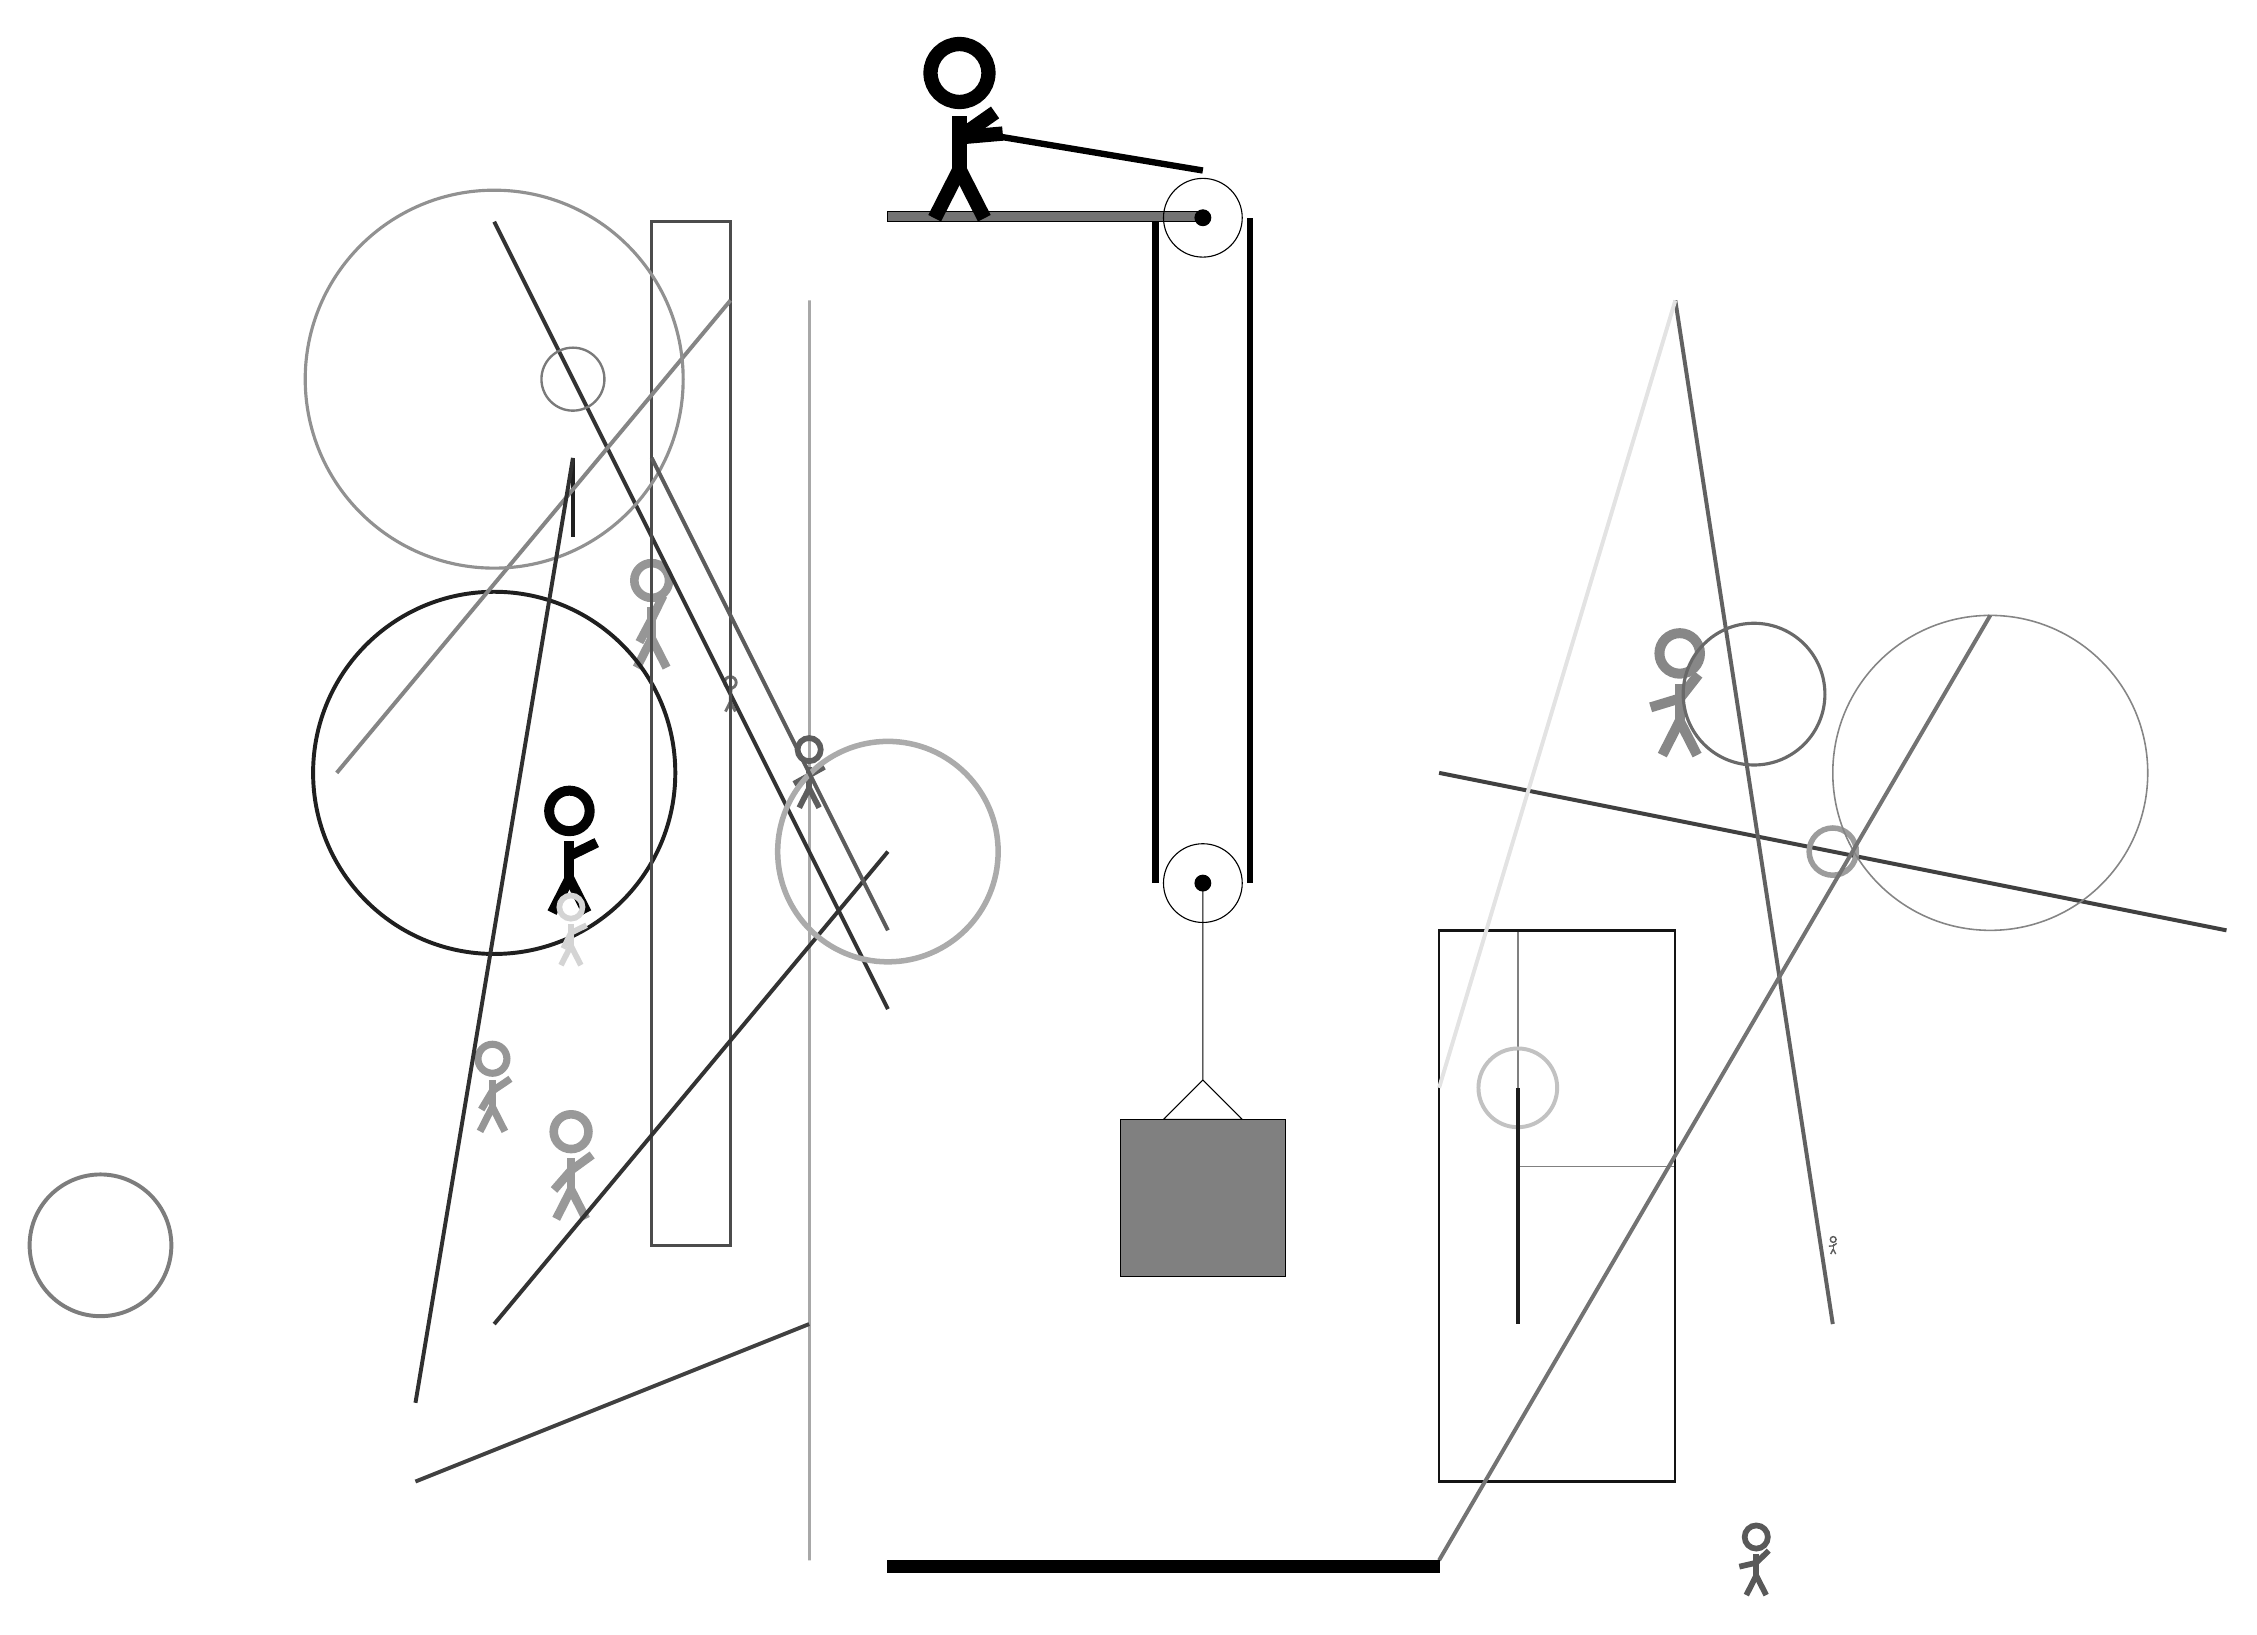
\begin{tikzpicture}
			%%%%% START %%%%%
			
			\draw[fill=black!55] (-2, 14) rectangle (2, 14.125);
			
			\draw (2, 5.6) circle (0.5);
			\draw[fill=black] (2, 5.6) circle (0.1);
			
			\draw (2, 14.05) circle (0.5);
			\draw[fill=black] (2, 14.05) circle (0.1);
			
			\node[line width=0.2mm, color=black!41] at (-5, 9) {\Strichmaxerl[6][62][64]};
			
			\node[line width=0.2mm, color=black!57] at (-4, 8) {\Strichmaxerl[2][88][83]};
			\draw [line width=0.3mm, color=black!44](-5, 2) circle (0.0);
			\draw [line width=0.5mm, color=black!88](-7, 7) circle (2.3);
			
			\node[line width=0.5mm, color=black!41] at (-7, 3) {\Strichmaxerl[5][59][34]};
			
			\node[line width=0.2mm, color=black!47] at (8, 8) {\Strichmaxerl[7][17][52]};
			\node[line width=0.6mm, color=black!40] at (-6, 2) {\Strichmaxerl[6][49][36]};
			\draw[line width=0.5mm, color=black!88](-6, 11) -- (-6, 10);
			\draw[line width=0.5mm, color=black!75](5, 7) -- (15, 5);
			
			\draw[line width=0.2mm, color=black!50] (6, 2) rectangle (8, 5);
			
			\draw[line width=0.5mm, color=black!62](10, 0) -- (8, 13);
			\draw[line width=0.4mm, color=black!34] (-3, 13) rectangle (-3, -3);
			\draw[line width=0.5mm, color=black!80](-7, 14) -- (-2, 4);
			
			\draw[line width=0.3mm, color=black!92] (5, 5) rectangle (8, -2);
			\draw[line width=0.4mm, color=black!70] (-4, 14) rectangle (-5, 1);
			\draw[line width=0.5mm, color=black!48](-4, 13) -- (-9, 7);
			
			\draw[line width=0.5mm, color=black!11](8, 13) -- (5, 3);
			
			\draw [line width=0.4mm, color=black!43](-7, 12) circle (2.4);
			\draw[line width=0.5mm, color=black!81](-6, 11) -- (-8, -1);
			\node[line width=0.6mm, color=black!63] at (10, 1) {\Strichmaxerl[1][2][37]};
			\draw [line width=0.5mm, color=black!24](6, 3) circle (0.5);
			\node[line width=0.2mm, color=black!99] at (-6, 6) {\Strichmaxerl[7][90][26]};
			
			\draw[line width=0.5mm, color=black!75](-3, 0) -- (-8, -2);
			\node[line width=0.2mm, color=black!17] at (-6, 5) {\Strichmaxerl[4][64][26]};
			\draw[line width=0.5mm, color=black!89](6, 3) -- (6, 0);
			
			\draw [line width=0.7mm, color=black!39](10, 6) circle (0.3);
			
			\node[line width=0.4mm, color=black!65] at (9, -3) {\Strichmaxerl[4][13][44]};
			\draw [line width=0.3mm, color=black!52](-6, 12) circle (0.4);
			\draw [line width=0.2mm, color=black!48](12, 7) circle (2.0);
			
			\draw[line width=0.5mm, color=black!55](5, -3) -- (12, 9);
			\draw [line width=0.4mm, color=black!59](9, 8) circle (0.9);
			
			\draw [line width=0.5mm, color=black!51](-12, 1) circle (0.9);
			\draw[line width=0.5mm, color=black!80](-7, 0) -- (-2, 6);
			
			\node[line width=0.3mm, color=black!63] at (-3, 7) {\Strichmaxerl[4][29][29]};
			
			\draw [line width=0.7mm, color=black!33](-2, 6) circle (1.4);
			\draw[line width=0.5mm, color=black!64](-2, 5) -- (-5, 11);
			
			
			\draw (2, 5.6) -- (2, 3.1) -- (1.5, 2.6) -- (2.5, 2.6) -- (2, 3.1);
			\draw[fill=black!50] (0.95, 2.6) rectangle (3.05, 0.6);
			
			\draw[line width=0.8mm] (1.4, 14) -- (1.4, 5.6);
			\centerarc[line width=0.8mm](2, 5.6)(180:360:0.6);
			\draw[line width=0.8mm](2.6, 5.6) -- (2.6, 14.05);
			\centerarc[line width=0.8mm](2, 14.05)(0:90:0.6);
			\draw[line width=0.8mm](2, 14.65) -- (-1, 15.15);
			
			\node at (-1, 15.15) {\Strichmaxerl[10][-175][35]};
			
			\draw[fill=black] (-2, -3) rectangle (5, -3.15);
			
			%%%%% END %%%%%
		\end{tikzpicture}
	\end{figure}	
\end{document}